\documentclass[aspectratio=169]{beamer}
\setbeamertemplate{navigation symbols}{}
\usepackage{color, amsmath, comment, subfigure}
\usepackage{url}
\usepackage{hyperref}
\hypersetup{
    colorlinks=true,
    linkcolor=blue,
    filecolor=magenta,      
    urlcolor=cyan,
}

%%%%%%%%%%%%%%%%%%%%%%%%%%
\title[]{Pre-read for Tuesday, Sept 8:\\
Predicting geopolitical events, part 1}
\author[]{Matthew J. Salganik}
\institute[]{}
\date[]{COS 597E/SOC 555 Limits to prediction\\Fall 2020, Princeton University}

\begin{document}
%%%%%%%%%%%%%%%%%%%%%%%%%%%
\frame{\titlepage}
%%%%%%%%%%%%%%%%%%%%%%%%%%%
\begin{frame}
\frametitle{}

Imagine:
\begin{itemize}
\item It is 1984
\pause
\item You've just gotten tenure at Berkeley
\pause 
\item You are sitting in a meeting at the National Research Council about the threat of nuclear war (also you are the youngest person there)
\pause
\item What is the probability of a nuclear war?
\pause
\item Everyone is making strong statements that often contradict each other, but you have no idea who is right.
\end{itemize}

\pause
What if we could systematically study political judgement? 

\end{frame}
%%%%%%%%%%%%%%%%%%%%%%%%%%%
\begin{frame}
\frametitle{}

\begin{center}
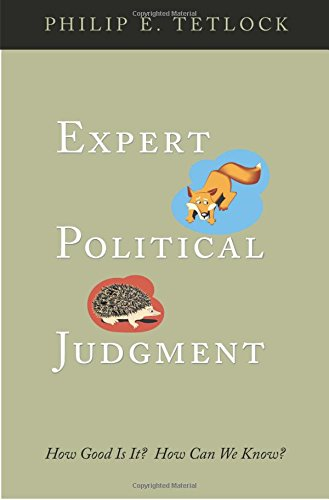
\includegraphics[height=0.7\textheight]{figures/tetlock_expert_2005_cover}
\end{center}

\vfill
20 years in the making

\end{frame}
%%%%%%%%%%%%%%%%%%%%%%%%%%%
\begin{frame}

``good political judgement''\\
\pause
Turning this idea into something measurable is hard.  This problem comes up often in social science.

\pause
Two focuses:
\begin{itemize}
\item accuracy (``Do they get it right?") 
\item rigor ("Do they think in the right way?")
\end{itemize}

\end{frame}
%%%%%%%%%%%%%%%%%%%%%%%%%
\begin{frame}

``good political judgement''\\
Turning this idea into something measurable is hard.  This problem comes up often in social science.

Two focuses:
\begin{itemize}
\item \textcolor{blue}{accuracy (``Do they get it right?")}
\item rigor ("Do they think in the right way?")
\end{itemize}

\end{frame}
%%%%%%%%%%%%%%%%%%%%%%%%%
\begin{frame}

Reading notes:
\begin{itemize}
\item Preface
\item Chapter 1, Quantifying the Unquantifiable
\item Chapter 2, The Ego-deflating Challenge of Radical Skepticism
\item Methodological Appendix, Section I: Regional Forecasting Exercises, Chapters 2 and 3
\item Technical Appendix, Part A: Correspondence Indicators of Good Judgement
\item Preface to the 2017 edition
\end{itemize}

\end{frame}
%%%%%%%%%%%%%%%%%%%%%%%%%%%
\begin{frame}

Preface:
\begin{itemize}
\item Notice how his research questions comes from his own personal annoyances and experiences.
\pause
\item How might this strategy be related to the projects that you will do in this class? What are the risks and benefits of this strategy for finding research topics?
\pause
\item If many academics follow this strategy (and I think they do) and if researchers do not match broader populations, what implications might there be for the kinds of questions that get studied and those that don't?
\end{itemize}

\end{frame}
%%%%%%%%%%%%%%%%%%%%%%%%%%%
\begin{frame}

Chapter 1:
\begin{itemize}
\item Notice that he is concern about the marketplace of ideas, not just predictive accuracy.
\pause
\item Splits ``good judgement'' into getting it right and thinking the right way.  We will focus on getting it right.
\pause
\item Beyond chapter 2 (which we won't read) has one of the most famous findings. You might ask what separates the more accurate forecasters from the less accurate.  It turns out that it is not background or political outlook, it is cognitive style.  He shows ``foxes'' who know lots of little things are better forecasters than ``hedgehogs'' who know one big thing.  Foxes and hedgehogs are on the cover of the book. 
\end{itemize}

\end{frame}
%%%%%%%%%%%%%%%%%%%%%%%%%%
\begin{frame}

Chapter 2:
\begin{itemize}
\item Notice reasons Tetlock presents for why experts might be bad at forecasting geo-political events; some are properties of the world and some of humans.  Pay attention to the ones that properties of the world because we will see them again in different forms this semester.
\pause
\item Notice how Tetlock turns the radical skeptics ideas into 6 testable hypotheses. But also notice that the linkage is not very tight; the hypotheses don't help us distinguish between how much of unpredictability comes from punctuated equillibra or game theory.
\pause
\item Notice what data Tetlock chooses to create in order to test his hypotheses.
\pause
\item Tetlock pays a lot of attention to which types of errors occur (eg, Fig 2.6 over-predict low probability events and under-predict high probability events).  Think a bit about how this teaches us something important beyond just accuracy.  This is a theme we will see again.
\pause
\item I recommend you flip back and forth between Methodological and Technical appendix.  Otherwise the empirical results are hard to understand.
\end{itemize}

\end{frame}
%%%%%%%%%%%%%%%%%%%%%%%%%%
\begin{frame}

Technical appendix:
\begin{itemize}
\item For our class, key part is page 273 - 283
\pause
\item If I give you some predictions you should be able to calculate what Tetlock calls ``probability score'' and ``variability, calibration, and discrimination''.
\pause
\item A theme we will see often is expert vs.\ simple algorithm vs.\ complex algorithm.  Note how Tetlock creates simple and complex algorithms.
\pause
\item Pay less attention (unless you are interested) to section ``Adjustments of probability scores to address conceptual objections'' except section ``Controversy-adjusted probability scores'' where he points out that 15\% of the outcomes are unclear.
\end{itemize}

\end{frame}
%%%%%%%%%%%%%%%%%%%%%%%%%%
\begin{frame}

Preface to the 2017 edition:
\begin{itemize}
\item It is neat to see how people reflect on their work after it has been out in the world
\end{itemize}

\end{frame}
%%%%%%%%%%%%%%%%%%%%%%%%%%
\begin{frame}

\begin{center}
\LARGE{Additional material}
\end{center}

\end{frame}
%%%%%%%%%%%%%%%%%%%%%%%%%%%
\begin{frame}

Possible Futures Study

\end{frame}
%%%%%%%%%%%%%%%%%%%%%%%%%%%
\begin{frame}

``Although political forecasting is obviously an inexact science, educated guesswork is still critical for setting priorities and making contingency plans. Your answers to the forecasting questions posed here will not be traceable either to you personally or to any institution with which you may be affiliated. Our goal is not to proclaim ‘winners’ and ‘losers’ in a forecasting contest but rather to study how highly trained professionals reason about complex real-world processes under conditions of uncertainty.''

\end{frame}
%%%%%%%%%%%%%%%%%%%%%%%%%%%
\begin{frame}

Part 1: Questions about your professional background, preferred style of thinking, and ideological and theoretical commitments.

\end{frame}
%%%%%%%%%%%%%%%%%%%%%%%%%%%
\begin{frame}

Part 2: Questions inside your area of expertise

\end{frame}
%%%%%%%%%%%%%%%%%%%%%%%%%%%
\begin{frame}

For Vietnam:
\begin{itemize}
\item Should we expect---over the next 2 years---increases, decreases, or essentially no changes in the marginal tax rate?
\end{itemize}

\begin{center}
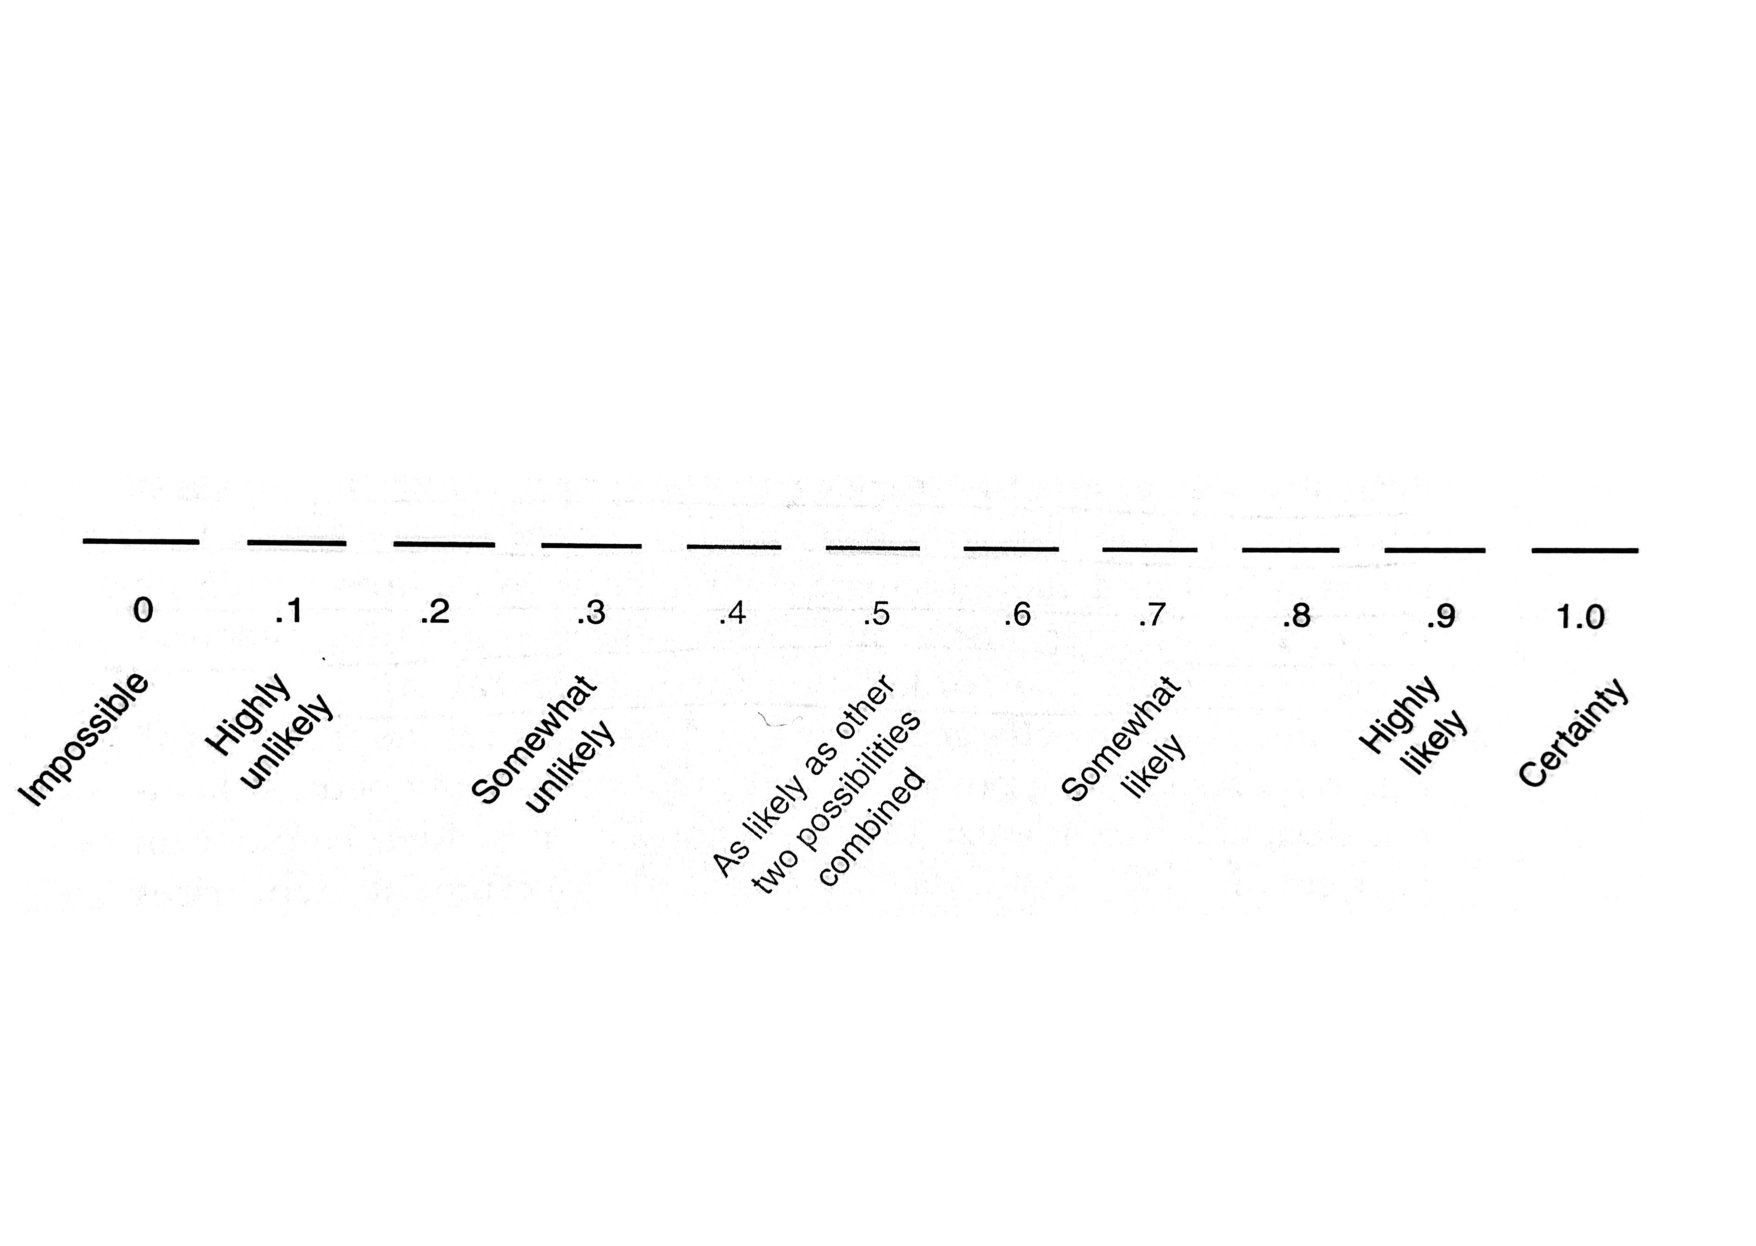
\includegraphics[width=\textwidth]{figures/tetlock_scale}
\end{center}

\pause

\begin{itemize}
\item Think of spreading probability over three buckets, not making a point prediction
\item Option to select ``maximum uncertainty'', which put 0.33 weight in each category (dart throwing chimp)
\end{itemize}

\end{frame}
%%%%%%%%%%%%%%%%%%%%%%
\begin{frame}

For Vietnam:
\begin{itemize}
\item Should we expect---over the next 2 years---increases, decreases, or essentially no changes in the marginal tax rate?
\item Should we expect---over the next 5 years---increases, decreases, or essentially no changes in the marginal tax rate?
\item Should we expect---over the next 5 years---defense spending as a percentage of central government expenditure to rise, fall, or stay the same?
\item Should we expect---over the next 10 years---defense spending as a percentage of central government expenditure to rise, fall, or stay the same?
\end{itemize}

\end{frame}
%%%%%%%%%%%%%%%%%%%%%%
\begin{frame}

Part 3: Questions outside your area of expertise

\end{frame}
%%%%%%%%%%%%%%%%%%%%%%%%%%%
\begin{frame}

Four content categories:
\begin{itemize}
\item continuity of domestic political leadership (eg, In the next election [Two elections from now], will the party with the most seats in the legislature keep that status, lose that status, or strengthen its position?)
\pause
\item domestic policy and economic performance (eg, Should we expect---over the next two years [or five years]---increases, decreases, or essentially no changes in the marginal tax rate?)
\pause
\item national security and defense policy (eg, Should we expect---over the next 5 years [or 10 years]---defense spending as a percentage of central government expenditure to rise, fall, or stay the same?)
\pause
\item special-purpose exercises (eg, weapons of mass destruction, Persian Gulf War I, etc.)
\end{itemize}

\pause
These questions were given at many different times to many different people so I don't think there is a single questionnaire.

\end{frame}
%%%%%%%%%%%%%%%%%%%%%%%%%%%
\begin{frame}

Notes about data:
\begin{itemize}
\item Probabilities are categorical (eg, 0, 0.1, 0.2) not continuous (eg, 0.2369), which impacts scoring
\pause
\item Outcomes generally split into three groups: increase, stay the same ($\pm$ 1 standard deviation), or down.  I'm not sure why it was set up that way.
\pause
\item There were many different exercises at different times so it is probably better to think of this as a collection of related studies rather than a single study
\end{itemize}

\end{frame}
%%%%%%%%%%%%%%%%%%%%%%%%%%%
\begin{frame}

What to read next?
\begin{itemize}
\item Readings for class on Thursday
\item More work by Tetlock and colleagues: \url{https://www.sas.upenn.edu/tetlock/}
\item Watch Tetlock's \href{https://www.youtube.com/watch?v=f73A-HB-08M}{book talk at Google}
\item Murphy (1973) \href{https://doi.org/10.1175/1520-0450(1973)012<0595:ANVPOTs>2.0.CO;2}{A New Vector Partition of the Probability Score}
\item Blattenberg and Lad (1985) \href{https://dx.doi.org/10.1080/00031305.1985.10479382}{Separating the Brier Score into Calibration and Refinement Components: A Graphical Exposition}
\item Murphy and Winkler (1987) \href{https://doi.org/10.1175/1520-0493(1987)115\%3C1330:AGFFFV\%3E2.0.CO;2}{A General Framework for Forecast Verification}
\end{itemize}

\end{frame}
%%%%%%%%%%%%%%%%%%%%%%%%%%%
\frame{\titlepage}

\end{document}
